Ahora se mostraran los procesos y el funcionamiento interno de la aplicación, los metodos, funciones, estructuras y clases.

La manera en que funcioanra la aplicación, com ya se menciono sera con una interfaz gráfica para el usuario, la cual estara comunicandose
con el modelo de la aplicación. La disposicion en la figura \ref{fig:UIDiagrama} una idea de la disposicion de la interfaz gráfica.
\begin{figure}[ht]
    \label{fig:UIDiagrama}
    \caption{Disposicion de la aplicación}
    \centering
    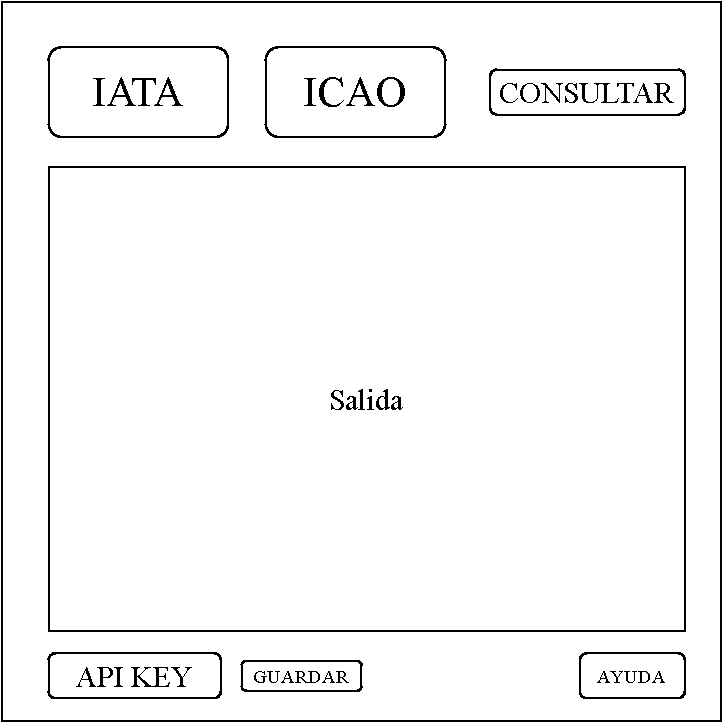
\includegraphics[width=\textwidth]{Figuras/UIDiagram.pdf}
\end{figure}

Las entradas serian los campos de AITA y IACO, mientras que tambien sera necesario que se proporcione una llave para la API, por lo
que seria otra entrada, ya que no es seguro incluir en el codigo, por lo que se requeria que el usuario proporcione su llave, tambien
se vera la posibilidad de guardar la llave en memoria para la comodidad del usuario.

Ahora pasando al modelo, veremos lo que lo va a conformar. Seguiremos el camino que seguiria los datos de entrada en el programa.

\subsection{Algoritmos}

Primero reciberemos la informacion recibida a travez de la interfaz, pero hay que tomar en cuanta que como tenemos 2 tipos de entrada, 
la IATA y la ICAO, por lo que se hara que la interfaz solo reciba 1 al mismo tiempo. Por otro lado recordemos que la API que se presento
en la sección \ref{subsec:API} de Arsenal, funciona con ICAO, no IATA, por lo que deberemos transformar el codigo IATA a ICAO.

\begin{algorithm}
    \caption{Tranforma de IATA a ICAO}\label{alg:IATA_TO_IACO}
    \begin{algorithmic}
        \Require Codigo IATA
        \State Transformar de IATA a ICAO \Comment{Aun no esta implementado}\\
        \Return Codigo ICAO
    \end{algorithmic}
\end{algorithm}

Despues de conseguir el codigo ICAO, ya sea directamente del usuario o por medio del algoritmo \ref{alg:IATA_TO_IACO},
seguira segura hacer la consulta del clima, para esto se tendra la cache como un diccionario con llaves de tipo \texttt{String},
las cuales seran el codigo ICAO, y valor \texttt{Información del Clima}. Pero para esto defincamos primero como guardaremos la informacion. 
Sera en una estructura la cual guardara la los siguientes datos:

\textbf{Información del Clima}
\begin{itemize}
    \label{strc:info}
    \item Codigo ICAO
    \item Codigo IATA
    \item Barometro
    \item Nubes
    \item Humedad
    \item Coordenadas
    \item Locación
    \item Nombre
    \item Temperatura
    \item Visibilidad
    \item Viento
    \item Tiempo de solicitud
\end{itemize}

Se incluira esto debido a que incluye la informacion basica asi como un poco de avanzada que puede llegar a ser de utilida a pilotos, aprte
que la respuesta de la API en METAR, que es un formato para ver el clima actual, se ve de esta manera.

\begin{lstlisting}[language=json,firstnumber=1]
    {
  "results": 1,
  "data": [
    {
      "barometer": {
        "hg": 30.02,
        "hpa": 1017.0,
        "kpa": 101.66,
        "mb": 1016.62
      },
      "clouds": [
        {
          "code": "CLR",
          "text": "Clear skies"
        }
      ],
      "dewpoint": {
        "celsius": 21,
        "fahrenheit": 70
      },
      "elevation": {
        "feet": 3,
        "meters": 1
      },
      "flight_category": "VFR",
      "humidity": {
        "percent": 79
      },
      "icao": "KPIE",
      "observed": "2021-04-30T23:53Z",
      "raw_text": "KPIE 302353Z AUTO 31009KT 10SM CLR 25/21 A3002 RMK AO2 SLP165 T02500206 10300 20250 55001",
      "station": {
        "geometry": {
          "coordinates": [
            -82.687401,
            27.9102
          ],
          "type": "Point"
        },
        "icao": "KPIE",
        "location": "St Petersburg-Clearwater, FL, USA",
        "name": "St Petersburg Clearwater International Airport",
        "type": "Airport"
      },
      "temperature": {
        "celsius": 25,
        "fahrenheit": 77
      },
      "visibility": {
        "meters": "16,000",
        "meters_float": 16000,
        "miles": "10",
        "miles_float": 10.0
      },
      "wind": {
        "degrees": 310,
        "speed_kph": 17,
        "speed_kts": 9,
        "speed_mph": 10,
        "speed_mps": 5
      }
    }
  ]
}
\end{lstlisting}

Ahora ya podemos pasar a ver como consultaremos el clima de un lugar. Este estara contenido en una estructura la cual sera la encargada
de manejar la informacion dependiendo de lo que se le vaya solicitando la que tenga el diccionario con todos los climas.
Tendra nadamas 2 atributos, ambos privados, los cuales seran el diccionario.
\texttt{InformacionClimas} prevamiente mencionado y la llave de la API.

\begin{algorithm}
    \caption{Algorimo para conseguir la informacion de clima de un lugar}\label{alg:prosClima}
    \begin{algorithmic}
        \Require Codigo ICAO(ICAO), Llave de API(API\_KEY)
        \State \texttt{solicitud\_actual} $\gets$ \texttt{InformacionClimas[ICAO]}
        \If{\texttt{solicitud\_actual} no existe o es muy vieja}
            \State $x \gets$ peticioAPI \Comment{PeticionAPI sera otra funcion dentro de la estructura}
            \If{La llamada fue exitosa}\\
                \State \texttt{solicitud\_actual} $\gets x$ 
            \Else\\
                \Return Llamada a la API fallida
            \EndIf
        \EndIf\\
        \Return \texttt{solicitud\_actual}
    \end{algorithmic}
\end{algorithm}


La llamda de la API tambien sera otra privada funcion dentro de la estructura que controlara toda la información. Por lo que reciberiamos la entrada
con lo que despues la procesariamos principalmente con el algoritmo \ref{alg:prosClima} para despues pasar lo obtenido a la interfaz, para que
asi sea desplegda al usuario. Tambien hay que recalcar que hay que pasar la información de la peticion hacia API, a la estructura definida previamente
para que de esta manera la aplicación entienda los datos, esto se hace de manera relativamente sencilla con las herramientas que ya nos
proporcina Swift como un JSONDecoder.